\documentclass[10pt,conference,compsoc]{IEEEtran}

\usepackage{amsmath}
\usepackage{bm}
\usepackage{float}
\usepackage{graphicx}
\PassOptionsToPackage{hyphens}{url}
  \usepackage[colorlinks=true,linkcolor=blue]{hyperref}
\usepackage{import}
\usepackage{listings}
\usepackage{tabulary}
\usepackage{tikz}

\newcommand{\includecode}[2][c]{%
  \lstinputlisting[escapechar=, style=custom#1]{#2}
}

% Load after hyperref
\usepackage[style=super,nonumberlist,toc]{glossaries}
\usepackage[notlof, notlot, nottoc]{tocbibind}
\usepackage{tocloft}

% Set up snippet environment
\newcommand{\listsnippetsname}{\Large List of Snippets}
\newlistof{snippets}{los}{\listsnippetsname}
\cftsetindents{snippets}{\parindent}{1.5\parindent}
\newenvironment{snippet}{
  \renewcommand{\caption}[1]{
    \refstepcounter{snippets}
    \begin{center}
      \par\noindent{\footnotesize Snippet \thesnippets. ##1}
    \end{center}
    \addcontentsline{los}{snippets}
      {\protect \numberline{\thesnippets}{\ignorespaces ##1}}
  }
}
{\par\noindent}

% Set styles for TikZ objects
\usetikzlibrary{arrows, positioning, shapes}
\tikzstyle{block} = [draw, rectangle, minimum height=3em, minimum width=4em]
\tikzstyle{sum} = [draw, circle, node distance=1cm]
\tikzstyle{arrow} = [arrows=->, black, align=right]
\tikzstyle{branch} = [circle, inner sep=0pt, minimum size=1mm, fill=black,
    draw=black]

\makeglossaries

\newcommand{\mtx}[1] {\bm #1}

% Disable automatic indent and provide \indent command
\newlength\tindent
\setlength{\tindent}{\parindent}
\setlength{\parindent}{0pt}
\renewcommand{\indent}{\hspace*{\tindent}}

\lstdefinestyle{customMatlab}{
  language=Matlab,
  breaklines=true,
  xleftmargin=0.125in,
  basicstyle=\footnotesize\ttfamily,
  keywordstyle=\color{blue},
  morekeywords=[2]{1}, keywordstyle=[2]{\color{black}},
  identifierstyle=\color{black},
  stringstyle=\color[RGB]{170, 55, 241},
  commentstyle=\color[RGB]{28, 172, 0},
  showstringspaces=false,
  emph=[1]{for,end,break},emphstyle=[1]\color{red},
}

\lstdefinestyle{customcpp}{
  belowcaptionskip=1\baselineskip,
  breaklines=true,
  xleftmargin=0.125in,
  language=C++,
  showstringspaces=false,
  basicstyle=\footnotesize\ttfamily,
  keywordstyle=\color[RGB]{128, 128, 0},
  commentstyle=\color[RGB]{0, 128, 0},
  identifierstyle=\color{black},
  stringstyle=\color[RGB]{0, 128, 0},
}

% Paper header
\usepackage{fancyhdr}
\pagestyle{fancy}
\lhead{Practical Guide to State-space Control}
\rhead{\thepage}
\lfoot{}
\rfoot{}
\fancyfoot[C]{}  % remove normal page numbers

\allowdisplaybreaks

\begin{document}
\input{INP-00-glossary}

\begin{titlepage}
  \begin{center}
    \vspace*{1cm}

    \Huge
    \textbf{Practical Guide to State-space Control}

    \vspace{0.5cm}
    \LARGE
    Graduate-level control theory for high schoolers

    \vspace{1.5cm}

    \textbf{Tyler Veness}

    \vfill

    \vspace{0.8cm}

    %\begin{figure}[H]
    %  \centering
    %  \def\svgwidth{0.25\columnwidth}
    %  \import{figs/}{wpilib.pdf_tex}
    %\end{figure}
  \end{center}

  \vfill


  \vspace{0.8cm}
\end{titlepage}
\thispagestyle{empty}  % no page number on title sheet

\pagenumbering{roman}
\renewcommand\contentsname{Table of Contents}
\tableofcontents
\listoffigures
\listoftables
\listofsnippets
\thispagestyle{empty}  % no page number on table of contents sheet
\clearpage

\pagenumbering{arabic}

\section*{Acknowledgements}

I would like to thank my controls engineering instructors Dejan Milutinovi\'c
and Gabriel Elkaim of University of California, Santa Cruz. They taught their
classes from a pragmatic perspective focused on application and intuition that I
appreciated. I would also like to thank Dejan Milutinovi\'c for introducing me
to the field of control theory and teaching me what it means to be a controls
engineer.

\section{Preface}

\subsection{Motivation}

I am the software mentor for a FIRST Robotics Competition team. My
responsibilities for that include teaching programming, software engineering
practices, and applications of control theory. The curriculum I developed so far
(located at \url{https://csweb.frc3512.com/ci/}) teaches rookies enough to be
minimally competitive, but many of the more advanced sections are incomplete. It
provides no formal avenues of growth for veteran students. \\

This project expands my curriculum to cover control theory topics I have learned
in my graduate-level engineering classes at University of California,
Santa Cruz. It introduces state-space controllers and serves as a practical
guide for formulating and implementing them. State-space control is a way of
formulating control problems using linear algebra that has several advantages
over simpler, typically heuristic approaches like
Proportional-Integral-Derivative (PID). \\

The sections on classical control theory are intended to provide a geometric
intuition into the mathematical machinery. Some topics have been oversimplified
to make them easier to grasp. For more detail, please see the Wikibook on
control systems at \url{https://en.wikibooks.org/wiki/Control_Systems}.

\subsection{Abstract}

Control theory is a discipline that deals with the behavior of dynamical
\glspl{system} with inputs, and how their behavior is modified by feedback.
Topics from classical and modern control are introduced, and advice is given on
when and how to apply them.

\subsection{Intended Audience}

This guide is intended to make an advanced engineering topic approachable so it
can be applied by those who aren't experts in control theory. My intended
audience is high school students who are returning veteran members of a FIRST
Robotics Competition team. As such, they will already be familiar with feedback
control applications like PID and have basic proficiency in programming. This
guide will build on their current knowledge of control theory and teach them
enough about state-space control and auxiliary topics to be able to implement it
in the programming language of their choice.

\section{What is control theory?}

How can we prove an autonomous car will behave safely? Control theory is used to
analyze and predict \gls{system} behavior. It's a pragmatic application of
algebra, geometry, and jargon with the goal of producing a desired \gls{system}
response. Feedback control facilitates producing a desired \gls{system}
response. Control theory involves judiciously expending engineering effort to
meet performance specifications.

\section{Nomenclature}

Most resources for advanced engineering topics assume a level of knowledge well
above that which is necessary. See the glossary for a list of words and phrases
commonly used in control theory, their origins, and their meaning. \\

For example, the \glspl{state} for a DC brushed motor would include the angular
velocity $\dot{\theta}$ and current $i$. Voltage $V$ is an input. With perfect
knowledge of the angular velocity and current, all future \glspl{state} of the
\gls{system} can be predicted given an input voltage signal.

\section{Control system diagrams}

\subsection{What is gain?}

Gain is a proportional value that shows the relationship between the magnitude
of the input to the magnitude of the output signal at steady state. Many
\glspl{system} contain a method by which the gain can be altered, providing more
or less "power" to the \gls{system}. However, increasing gain or decreasing gain
beyond a particular safety zone can cause the \gls{system} to become unstable.

\subsection{Block diagrams}

When designing or analyzing a control system, it is useful to model it
graphically. Block diagrams are used for this purpose. They can be manipulated
and simplified systematically \cite{bib:block_diagrams}. Figure
\ref{fig:feedback_loop} is an example of one with a feedback configuration.

\begin{figure}[H]
  \centering

  \begin{tikzpicture}[auto, >=latex']
    % Place the blocks
    \node [name=input] {$X(s)$};
    \node [sum, right=of input] (sum) {};
    \node [block, right=of sum] (P1) {$P_1$};
    \node [right=of P1] (output) {$Y(s)$};
    \node [block, below=of P1] (P2) {$P_2$};

    % Connect the nodes
    \draw [arrow] (input) -- node[pos=0.85] {$+$} (sum);
    \draw [arrow] (sum) -- node {} (P1);
    \draw [arrow] (P1) -- node[name=y] {} (output);
    \draw [arrow] (y) |- (P2);
    \draw [arrow] (P2) -| node[pos=0.97, right] {$\mp$} (sum);
  \end{tikzpicture}

  \caption{Feedback block diagram}
  \label{fig:feedback_loop}
\end{figure}

\section{Review of PID controller mathematics}

\subsection{PID basics and theory}

Negative feedback loops drive the difference between \gls{reference} and
\gls{output} to zero. \\

\textbf{Proportional} gain compensates for current \gls{error}. \\
\textbf{Integral} gain compensates for past error (i.e.,
\gls{steady-state error}). \\
\textbf{Derivative} gain compensates for future error by slowing controller down
  if error decreases over time.

\begin{figure}[H]
  \centering

  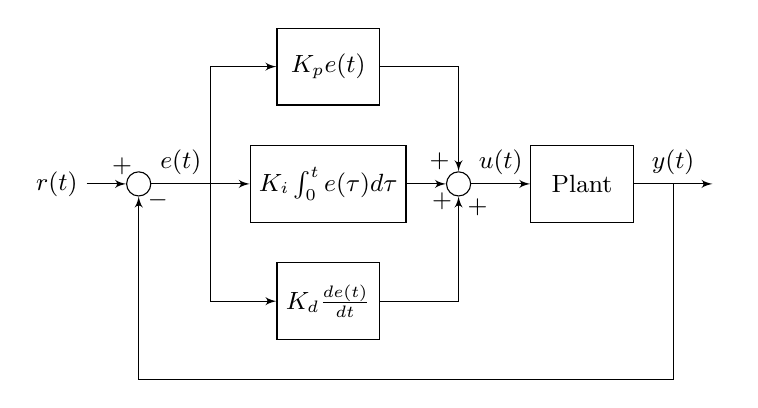
\begin{tikzpicture}[auto, >=latex']
    \fontsize{9pt}{10pt}

    % Place the blocks
    \node [name=input] {$r(t)$};
    \node [sum, right=0.5cm of input] (errorsum) {};
    \node [coordinate, right=0.75cm of errorsum] (branch) {};
    \node [block, right=0.5cm of branch] (I) { $K_i \int_0^t e(\tau) d\tau$ };
    \node [block, above=0.5cm of I] (P) { $K_p e(t)$ };
    \node [block, below=0.5cm of I] (D) { $K_d \frac{de(t)}{dt}$ };
    \node [sum, right=0.5cm of I] (ctrlsum) {};
    \node [block, right=0.75cm of ctrlsum] (plant) {Plant};
    \node [right=of plant] (output) {};
    \node [coordinate, below=0.5cm of D] (measurements) {};

    % Connect the nodes
    \draw [arrow] (input) -- node[pos=0.9] {$+$} (errorsum);
    \draw [-] (errorsum) -- node {$e(t)$} (branch);
    \draw [arrow] (branch) |- (P);
    \draw [arrow] (branch) -- (I);
    \draw [arrow] (branch) |- (D);
    \draw [arrow] (P) -| node[pos=0.95, left] {$+$} (ctrlsum);
    \draw [arrow] (I) -- node[pos=0.9, below] {$+$} (ctrlsum);
    \draw [arrow] (D) -| node[pos=0.95, right] {$+$} (ctrlsum);
    \draw [arrow] (ctrlsum) -- node {$u(t)$} (plant);
    \draw [arrow] (plant) -- node [name=y] {$y(t)$} (output);
    \draw [-] (y) |- (measurements);
    \draw [arrow] (measurements) -| node[pos=0.99, right] {$-$} (errorsum);
  \end{tikzpicture}

  \caption{PID controller diagram}
  \label{fig:pid_ctrl_diag}
\end{figure}

\begin{table}[ht]
  \renewcommand{\arraystretch}{1.3}
  \centering
  \begin{tabulary}{\linewidth}{LLLL}
    $r(t)$ & \gls{reference} input & $u(t)$ & control input \\
    $e(t)$ & error & $y(t)$ & \gls{output} \\
  \end{tabulary}
  \label{tab:pid_def}
\end{table}

\begin{table}[ht]
  \caption{Plant versus controller}
  \renewcommand{\arraystretch}{1.3}
  \centering
  \begin{tabular}{|l|ll|}
    \hline
    & \textbf{Plant} & \textbf{Controller} \\
    \hline
    Input & $u(t)$ & $r(t)$, $y(t)$ \\
    Output & $y(t)$ & $u(t)$ \\
    \hline
  \end{tabular}
  \label{tab:plant_v_controller}
\end{table}

\subsection{Types of PID controllers}

PID controller inputs of different orders of derivatives, such as position and
velocity, affect the \gls{system} response differently. The position PID
controller is defined as

\begin{equation}
  u(t) = K_p e(t) + K_i \int_0^t e(\tau) d\tau + K_d \frac{de}{dt} \\
\end{equation}
\\
If a velocity is passed instead, which is a change in position, the equation
becomes

\begin{align}
  \frac{du}{dt} &= K_p \frac{de}{dt} + K_i \int_0^t \frac{de}{d\tau} d\tau +
    K_d \frac{d^2e}{dt^2} \nonumber \\
  \frac{du}{dt} &= K_p \frac{de}{dt} + K_i e(t) + K_d \frac{d^2e}{dt^2}
    \label{eq:pid_vel}
\end{align}
\\
This shows that $K_i$ and $K_p$ from the position controller act as proportional
and derivative terms respectively in the velocity controller. $K_i$ from the
position controller has no equivalent in the velocity controller. If we were to
implement one, it would use a double integral. However, it would be of limited
use since the $K_i$ term in equation (\ref{eq:pid_vel}) also eliminates
steady-state error for step changes in \gls{reference}. Relabelling the
coefficients to match the position PID controller gives

\begin{equation}
  \frac{du}{dt} = K_p \int_0^t e(\tau) d\tau + K_d e(t) \\
\end{equation}
\\
Read \url{https://en.wikipedia.org/wiki/PID_controller} for more information.

\subsection{Limitations of PID control}

PID's heuristic method of tuning is fine when there is no knowledge of the
\gls{system}. However, controllers with much better response can be developed if
a dynamical model of the \gls{system} is known.

\section{What is a transfer function?}

A transfer function maps an input to an output in the Laplace domain. This is
essentially a two-dimensional frequency domain on the complex plane (real
numbers on the x-axis and imaginary numbers on the y-axis). These can be
obtained by applying the Laplace transform to a differential equation and
rearranging the terms to obtain a ratio of the output variable to the input
variable. Equation \ref{eq:transfer_func} is an example of a transfer function.

\begin{equation} \label{eq:transfer_func}
  H(s) = \frac{(s-9+9i)(s-9-9i)}{s(s+10)} \\
\end{equation}

Roots of the numerator and denominator are called residues. Residues on the top
are called zeroes while residues on the bottom are called poles. This is due to
poles making the expression approach infinity for values of $s$ that make the
residue zero (they look like poles of a circus tent on a 3D graph). Similar
logic applies to zeroes. Imaginary roots always come in complex conjugate pairs
(e.g., $-2 + 3i$, $-2 - 3i$).

\subsection{Transfer functions in feedback}

For \glspl{controller} to perform their job, they must be placed in positive or
negative feedback with the \gls{plant} (positive or negative depends on the
\gls{plant} in question). The transfer function of figure
\ref{fig:feedback_loop}, a control system diagram with feedback, from input to
output is

\begin{equation}
  G_{cl}(s) = \frac{Y(s)}{X(s)} = \frac{P_1}{1 + P_1 P_2}
\end{equation}

The numerator is the \gls{open-loop gain} and the denominator is the gain around
the feedback loop, which may include parts of the \gls{open-loop gain} (see
appendix \ref{sec:app_tf_feedback_deriv} for a derivation). Plants are generally
denoted with the letter $G$. As another example, the transfer function from the
input to the error is

\begin{equation}
  G_{cl}(s) = \frac{E(s)}{X(s)} = \frac{1}{1 + P_1 P_2}
\end{equation}

The roots of the denominator of $G_{cl}(s)$ are different from those of the
open-loop transfer function $P_1(s)$. These are called the closed-loop poles.

\section{Location of Poles and Zeroes}

The location of the closed-loop poles on the complex plane determine the
stability of the \gls{system}. Each pole represents a frequency mode of the
\gls{system}, and their location determines how much of each response is induced
for a given input frequency.

\begin{figure}[H]
  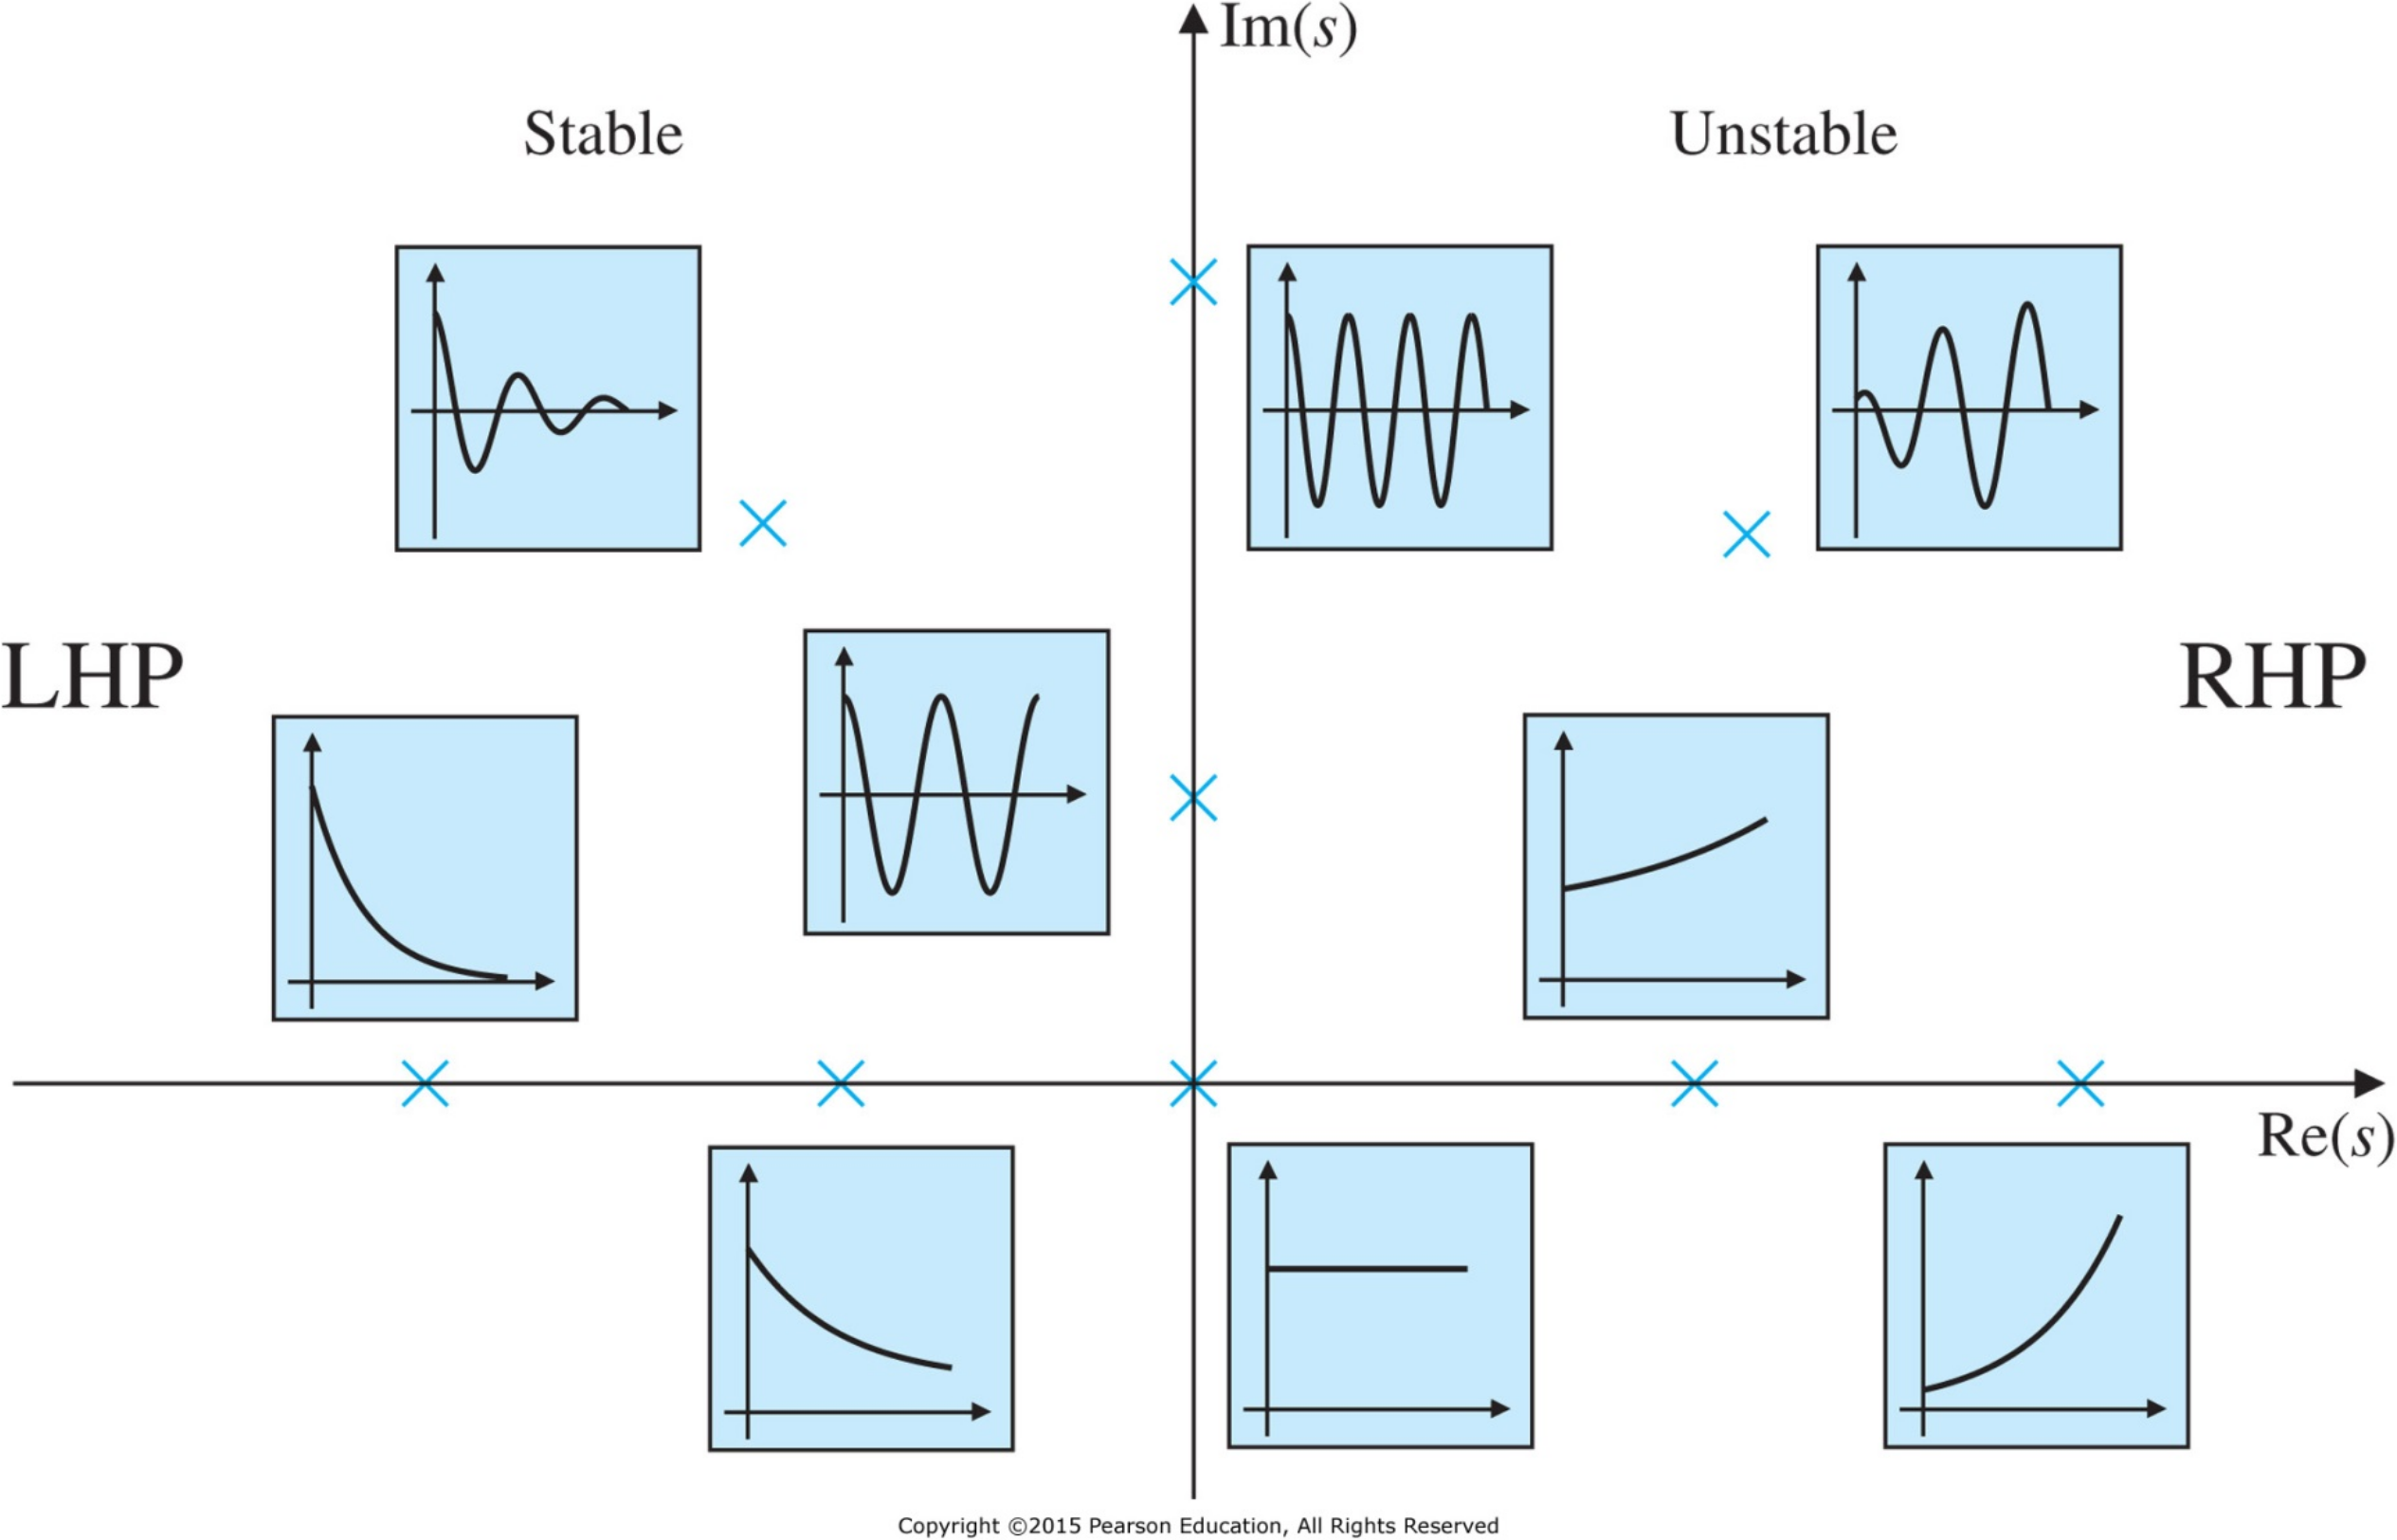
\includegraphics[width=\linewidth]{figs/ResponseVsPoleLocations.png}
  \caption{System responses vs pole locations \cite{bib:pole_locations}}
\end{figure}

\begin{table}[ht]
  \caption{Pole location and stabilty}
  \renewcommand{\arraystretch}{1.5}
  \centering
  \begin{tabular}{|ll|}
    \hline
    \textbf{Location} & \textbf{Stability} \\
    \hline
    Left-Hand Plane (LHP) & stable \\
    Imaginary Axis & marginally stable \\
    Right-Hand Plane (RHP) & unstable \\
    \hline
  \end{tabular}
  \label{tab:pole_locations}
\end{table}

\subsection{Root locus}

In closed-loop, the poles and zeroes can be moved around by the chosen
controller. The root locus shows where they will go as the controller gain is
increased. Figure \ref{fig:poster_rlocus} shows the root locus of the transfer
function from equation (\ref{eq:transfer_func}).

\begin{figure}[H]
  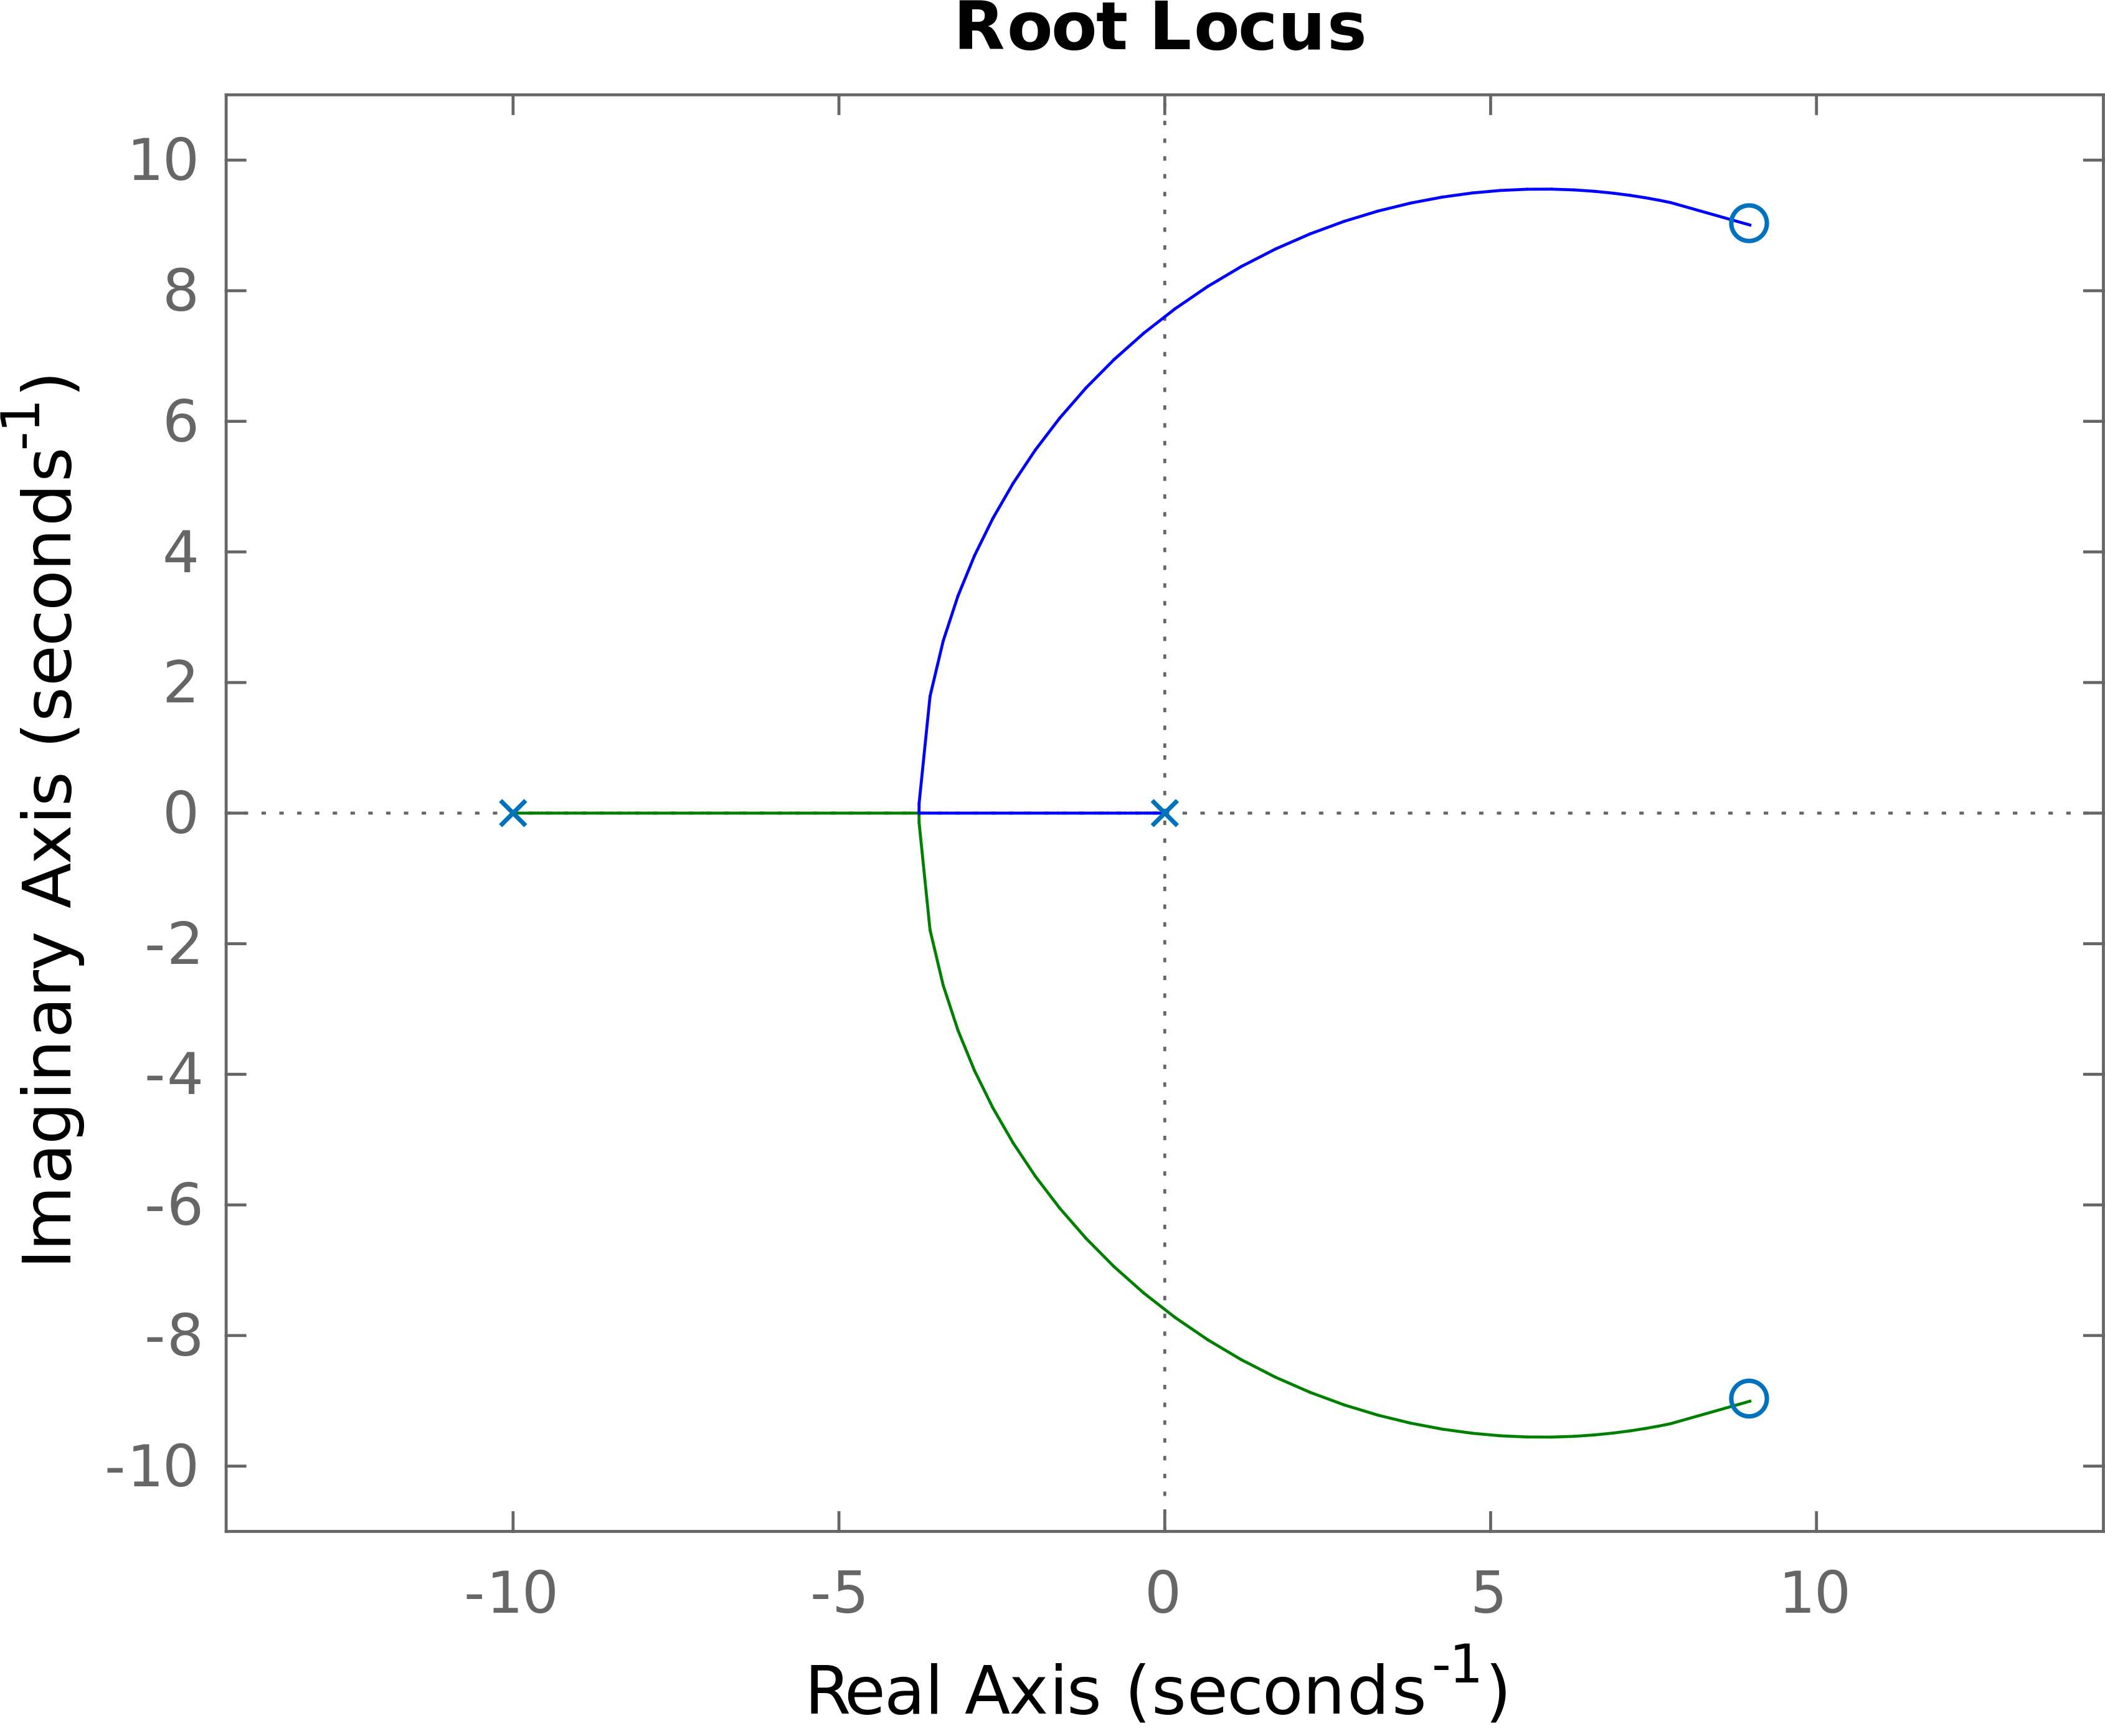
\includegraphics[width=\linewidth]{figs/poster_rlocus.png}
  \caption{Root locus of equation (\ref{eq:transfer_func}). See snippet
    \ref{snip:poster_rlocus}.}
  \label{fig:poster_rlocus}
\end{figure}

\begin{snippet}
  \caption{Root locus in MATLAB}
  \label{snip:poster_rlocus}
  \includecode[Matlab]{code/root_locus.m}
\end{snippet}

As the controller gain increases, the poles move toward the zeroes. In this
case, the \gls{system} eventually becomes unstable. \\

\textbf{Note:} If poles are much farther left in the LHP than the typical
\gls{system} dynamics exhibit, they can be considered negligible. Every
\gls{system} has some form of unmodeled high frequency, non-linear dynamics, but
they can be safely ignored depending on the operating regime.

\subsubsection{Non-minimum phase zeroes}

While poles in the RHP are unstable, the same is not true for zeroes. They can
be characterized by the \gls{system} initially moving in the wrong direction
before heading toward the \gls{reference}. Since the poles always move toward
the zeroes, zeroes impose a "speed limit" on the \gls{system} response because
it takes a finite amount of time to move the wrong direction, then change
directions. \\

One example is bicycle steering. Try riding a bicycle without holding the handle
bars, then poke the right handle; the bicycle turns right.

\section{Steady-state error}

To demonstrate the problem of \gls{steady-state error}, we will use a DC brushed
motor controlled by a velocity PID controller. A DC brushed motor has a transfer
function from voltage ($V$) to angular velocity ($\dot{\theta}$) of

\begin{equation}
  G(s) = \frac{\dot{\Theta}(s)}{V(s)} = \frac{K}{(Js+b)(Ls+R)+K^2} \\
\end{equation}

First, we'll try controlling it with a P controller defined as

\begin{equation*}
  K(s) = K_p \\
\end{equation*}

When these are in unity feedback, the transfer function from the input voltage
to the error is

\begin{align*}
  \frac{E(s)}{V(s)} &= \frac{1}{1 + K(s)G(s)} \\
  E(s) &= \frac{1}{1 + K(s)G(s)} V(s) \\
  E(s) &= \frac{1}{1 + (K_p) \left(\frac{K}{(Js+b)(Ls+R)+K^2}\right)} V(s) \\
  E(s) &= \frac{1}{1 + \frac{K_p K}{(Js+b)(Ls+R)+K^2}} V(s)
\end{align*}

The steady-state of a transfer function can be found via

\begin{equation}
  \lim_{s\to0} sH(s)
\end{equation}

\begin{align}
  e_{ss} &= \lim_{s\to0} sE(s) \nonumber \\
  e_{ss} &= \lim_{s\to0} s \frac{1}{1 + \frac{K_p K}{(Js+b)(Ls+R)+K^2}} V(s)
    \nonumber \\
  e_{ss} &= \lim_{s\to0} s \frac{1}{1 + \frac{K_p K}{(Js+b)(Ls+R)+K^2}}
    \frac{1}{s} \nonumber \\
  e_{ss} &= \lim_{s\to0} \frac{1}{1 + \frac{K_p K}{(Js+b)(Ls+R)+K^2}}
    \nonumber \\
  e_{ss} &= \frac{1}{1 + \frac{K_p K}{(J(0)+b)(L(0)+R)+K^2}} \nonumber \\
  e_{ss} &= \frac{1}{1 + \frac{K_p K}{bR+K^2}} \label{eq:ss_nonzero}
\end{align}

Notice that the \gls{steady-state error} is non-zero. To fix this, an integrator
must be included in the controller.

\begin{equation*}
  K(s) = K_p + \frac{K_i}{s} \\
\end{equation*}

The same steady-state calculations are performed as before with the new
controller.

\begin{align*}
  \frac{E(s)}{V(s)} &= \frac{1}{1 + K(s)G(s)} \\
  E(s) &= \frac{1}{1 + K(s)G(s)} V(s) \\
  E(s) &= \frac{1}{1 + \left(K_p + \frac{K_i}{s}\right)
    \left(\frac{K}{(Js+b)(Ls+R)+K^2}\right)} \left(\frac{1}{s}\right) \\
  e_{ss} &= \lim_{s\to0} s \frac{1}{1 + \left(K_p + \frac{K_i}{s}\right)
    \left(\frac{K}{(Js+b)(Ls+R)+K^2}\right)} \left(\frac{1}{s}\right) \\
  e_{ss} &= \lim_{s\to0} \frac{1}{1 + \left(K_p + \frac{K_i}{s}\right)
    \left(\frac{K}{(Js+b)(Ls+R)+K^2}\right)} \\
  e_{ss} &= \lim_{s\to0} \frac{1}{1 + \left(K_p + \frac{K_i}{s}\right)
    \left(\frac{K}{(Js+b)(Ls+R)+K^2}\right)} \frac{s}{s} \\
  e_{ss} &= \lim_{s\to0} \frac{s}{s + \left(K_p s + K_i\right)
    \left(\frac{K}{(Js+b)(Ls+R)+K^2}\right)} \\
  e_{ss} &= \frac{0}{0 + (K_p (0) + K_i)
    \left(\frac{K}{(J(0)+b)(L(0)+R)+K^2}\right)} \\
  e_{ss} &= \frac{0}{K_i \frac{K}{bR+K^2}} \\
\end{align*}

The denominator is non-zero, so $e_{ss} = 0$. Therefore, an integrator is
required to eliminate \gls{steady-state error} in all cases for this model. \\

It should be noted that $e_{ss}$ in equation (\ref{eq:ss_nonzero}) approaches
zero for $K_p = \infty$. This is known as a bang-bang controller. In practice,
an infinite switching frequency cannot be achieved, but it may be close enough
for some performance specifications.

\section{Going Digital}

The complex plane discussed so far deals with continuous \glspl{system}. In
decades past, \glspl{plant} and controllers were implemented using analog
electronics, which are continuous in nature. Nowadays, microprocessors can be
used to achieve cheaper, less complex controller designs. However, this comes
with drawbacks. \\

Since a microcontroller performs discrete steps, there is phase loss introduced
in the controller. Large amounts of phase loss can make a stable controller in
the continuous domain go unstable in discrete. Here are a few ways to combat
this.

\begin{itemize}
  \item Run the controller with a high sample rate.
  \item Designing the controller in the analog domain with enough phase margin
    to compensate for any phase loss that occurs as part of discretization.
  \item Convert the \gls{plant} to the digital domain and design the controller
    completely in the digital domain.
\end{itemize}

\subsection{s-plane to z-plane}

Transfer functions are converted to impulse responses using the Z-transform. The
s-plane's LHP maps to the inside of a unit circle in the z-plane. Here are a few
common points.

\begin{table}[ht]
  \caption{Mapping from s-plane to z-plane}
  \renewcommand{\arraystretch}{1.3}
  \centering
  \begin{tabular}{|cc|}
    \hline
    \textbf{s-plane} & \textbf{z-plane} \\
    \hline
    $(0, 0)$ & $(0, 1)$ \\
    imaginary axis & edge of unit circle \\
    $(0, -\infty)$ & $(0, 0)$ \\
    \hline
  \end{tabular}
  \label{tab:s-plane2z-plane}
\end{table}

You may notice that poles can be placed at $(0, 0)$ in the z-plane. This is
known as a deadbeat controller. An $\rm N^{th}$ order deadbeat controller decays
to the \gls{reference} in N timesteps. While this sounds great, there are other
considerations like actuation effort and robustness. These will be discussed in
detail with LQR controllers.

\section{Linear algebra}

Modern control theory borrows concepts from linear algebra. We recommend
watching 3Blue1Brown's \textit{Essence of Linear Algebra} video series
\cite{bib:essence_of_linalg}. It offers an intuitive, geometric understanding of
linear algebra as a method of linear transformations. \\

\textit{Note}: The $^T$ in $\mtx{A}^T$ denotes transpose, which flips the matrix
across its diagonal such that the rows become columns and vice versa.

\section{State-space}

A state-space representation models \glspl{system} as a set of \gls{state},
input, and output variables related by first-order differential equations.
"State space" refers to the Euclidean space in which the \gls{state} variables
are on the axes. The \gls{state} of the \gls{system} can be represented as a
vector within that space. \\

To abstract from the number of \glspl{state}, inputs, and outputs, these
variables are expressed as vectors. Additionally, if the dynamical \gls{system}
is linear, time-invariant, and finite-dimensional, then the differential and
algebraic equations may be written in matrix form.

\subsection{Benefits over classical output-based control}

The state-space method is characterized by significant algebraization of general
system theory. The state-space representation uses the time domain instead of
the frequency domain, and provides a convenient and compact way to model and
analyze \glspl{system} with multiple inputs and outputs. With $p$ inputs and $q$
outputs, we would otherwise have to write down $q \times p$ Laplace transforms
to encode all the information about a system. Unlike the frequency domain
approach, the use of the state-space representation is not limited to systems
with linear components and zero initial conditions.

\section{State-space notation}

\begin{align}
  \dot{\mtx{x}} &= \mtx{A}\mtx{x} + \mtx{B}\mtx{u} \label{eq:s_ctrl_x} \\
  \mtx{y} &= \mtx{C}\mtx{x} + \mtx{D}\mtx{u} \label{eq:s_ctrl_y}
\end{align}

\begin{align}
  \mtx{x}_{k+1} &= \mtx{A}\mtx{x}_k + \mtx{B}\mtx{u}_k \label{eq:z_ctrl_x} \\
  \mtx{y}_{k+1} &= \mtx{C}\mtx{x}_k + \mtx{D}\mtx{u}_k \label{eq:z_ctrl_y}
\end{align}

\begin{table}[ht]
  \renewcommand{\arraystretch}{1.3}
  \centering
  \begin{tabulary}{\linewidth}{LLLL}
    $\mtx{A}$ & system matrix      & $\mtx{x}$ & state vector \\
    $\mtx{B}$ & input matrix       & $\mtx{u}$ & input vector \\
    $\mtx{C}$ & output matrix      & $\mtx{y}$ & output vector \\
    $\mtx{D}$ & feedthrough matrix & $\mtx{K}$ & controller gain matrix \\
  \end{tabulary}
  \label{tab:ctrl_def}
\end{table}

\begin{table}[ht]
  \caption{State-space matrix dimensions}
  \renewcommand{\arraystretch}{1.5}
  \centering
  \begin{tabular}{|ll|}
    \hline
    \textbf{Matrix} & \textbf{Dimensions (rows $\times$ columns)} \\
    \hline
    $\mtx{A}$ & states $\times$ states \\
    $\mtx{B}$ & states $\times$ inputs \\
    $\mtx{C}$ & outputs $\times$ states \\
    $\mtx{D}$ & outputs $\times$ inputs \\
    $\mtx{x}$ & states $\times$ 1 \\
    $\mtx{u}$ & inputs $\times$ 1 \\
    $\mtx{y}$ & outputs $\times$ 1 \\
    $\mtx{K}$ & inputs $\times$ states \\
    \hline
  \end{tabular}
  \label{tab:ss_matrix_dims}
\end{table}

\section{Canonical forms}

There are two canonical forms used to represent state-space models: controllable
canonical form and observable canonical form. They are used to provide
controllability and observability of a system respectively, which are
mathematical duals of each other. That is, the controller and estimator (state
observer) are complementary problems.

\subsection{Controllable canonical form} \label{subsec:ctrl_canon}

State controllability implies that it is possible -- by admissible inputs -- to
steer the \glspl{state} from any initial value to any final value within some
finite time window. A continuous \gls{time-invariant} linear state-space model
is controllable if and only if

\begin{equation}
  rank \left[
  \begin{array}{ccccc}
    B & AB & A^2B & \cdots & A^{n-1}B
  \end{array}
  \right] = n
  \label{eq:ctrl_rank}
\end{equation}

where rank is the number of linearly independent rows in a matrix and $n$ is the
number of \gls{state} variables. \\

Given a \gls{system} of the form

\begin{equation} \label{eq:ctrl_obsv_tf}
  G(s) = \frac{n_1 s^3 + n_2 s^2 + n_3 s + n_4}
    {s^4 + d_1 s^3 + d_2 s^2 + d_3 s + d_4} \\
\end{equation}
\\
The canonical realization of it that satisfies equation (\ref{eq:ctrl_rank}) is

\begin{align}
  \dot{\mtx{x}}(t) &= \left[
  \begin{array}{cccc}
    0 & 1 & 0 & 0 \\
    0 & 0 & 1 & 0 \\
    0 & 0 & 0 & 1 \\
    -d_4 & -d_3 & -d_2 & -d_1
  \end{array}
  \right] \mtx{x}(t) + \left[
  \begin{array}{c}
    0 \\
    0 \\
    0 \\
    1
  \end{array}
  \right] \mtx{u}(t) \\
  \mtx{y}(t) &= \left[
  \begin{array}{cccc}
    n_4 & n_3 & n_2 & n_1
  \end{array}
  \right] \mtx{x}(t)
\end{align}

\subsection{Observable canonical form} \label{subsec:obsv_canon}

Observability is a measure for how well internal \glspl{state} of a \gls{system}
can be inferred by knowledge of its external outputs. The observability and
controllability of a \gls{system} are mathematical duals (i.e., as
controllability proves that an input is available that brings any initial
\gls{state} to any desired final \gls{state}, observability proves that knowing
an output trajectory provides enough information to predict the initial
\gls{state} of the \gls{system}). \\

A continuous \gls{time-invariant} linear state-space model is observable if and
only if

\begin{equation} \label{eq:obsv_rank}
  rank \left[
  \begin{array}{c}
    C \\
    CA \\
    \vdots \\
    CA^{n-1}
  \end{array}
  \right] = n \\
\end{equation}

The canonical realization of the \gls{system} in equation
(\ref{eq:ctrl_obsv_tf}) that satisfies equation (\ref{eq:obsv_rank}) is

\begin{align}
  \dot{\mtx{x}}(t) &= \left[
  \begin{array}{cccc}
    0 & 0 & 0 & -d_4 \\
    1 & 0 & 0 & -d_3 \\
    0 & 1 & 0 & -d_2 \\
    0 & 0 & 1 & -d_1
  \end{array}
  \right] \mtx{x}(t) + \left[
  \begin{array}{c}
    n_4 \\
    n_3 \\
    n_2 \\
    n_1
  \end{array}
  \right] \mtx{u}(t) \\
  \mtx{y}(t) &= \left[
  \begin{array}{cccc}
    0 & 0 & 0 & 1
  \end{array}
  \right] \mtx{x}(t)
\end{align}

\section{Eigenvalues in state-space}

Eigenvalues can be used to determine the stability of a \gls{system}. \\

We'd like to know whether the \gls{system} defined by equation
(\ref{eq:z_ctrl_x}) operating with the input
$\mtx{u}_k = \mtx{K}(\mtx{R}_k - \mtx{x}_k)$ converges to the \gls{reference}
$\mtx{R}_k$.

\begin{align}
  \mtx{x}_{k+1} &= \mtx{A}\mtx{x}_k + \mtx{B}\mtx{u}_k \nonumber \\
  \mtx{x}_{k+1} &= \mtx{A}\mtx{x}_k + \mtx{B}(\mtx{K}(\mtx{R}_k - \mtx{x}_k))
    \nonumber \\
  \mtx{x}_{k+1} &= \mtx{A}\mtx{x}_k + \mtx{B}\mtx{K}\mtx{R}_k -
    \mtx{B}\mtx{K}\mtx{x}_k \nonumber \\
  \mtx{x}_{k+1} &= \mtx{A}\mtx{x}_k - \mtx{B}\mtx{K}\mtx{x}_k +
    \mtx{B}\mtx{K}\mtx{R}_k \nonumber \\
  \mtx{x}_{k+1} &= (\mtx{A} - \mtx{B}\mtx{K})\mtx{x}_k +
    \mtx{B}\mtx{K}\mtx{R}_k \label{eq:ctrl_eig_calc}
\end{align}
\\
For equation (\ref{eq:ctrl_eig_calc}) to have a bounded output, the eigenvalues
of $\mtx{A} - \mtx{B}\mtx{K}$ must be within the unit circle. \\

This derivation can be performed for a \gls{state} estimator as well to
determine whether the \gls{state} estimate converges to the true \gls{state}.
Plugging equation (\ref{eq:z_obsv_y}) into equation (\ref{eq:z_obsv_x}) gives

\begin{align*}
  \hat{\mtx{x}}_{k+1} &= \mtx{A}\hat{\mtx{x}}_k + \mtx{B}\mtx{u}_k +
    \mtx{L} (\mtx{y}_k - \hat{\mtx{y}}_{k+1}) \\
  \hat{\mtx{x}}_{k+1} &= \mtx{A}\hat{\mtx{x}}_k + \mtx{B}\mtx{u}_k +
    \mtx{L} (\mtx{y}_k - (\mtx{C}\hat{\mtx{x}}_k + \mtx{D}\mtx{u}_k)) \\
  \hat{\mtx{x}}_{k+1} &= \mtx{A}\hat{\mtx{x}}_k + \mtx{B}\mtx{u}_k +
    \mtx{L} (\mtx{y}_k - \mtx{C}\hat{\mtx{x}}_k - \mtx{D}\mtx{u}_k) \\
\end{align*}

Plugging in equation (\ref{eq:z_ctrl_y}) gives

\begin{align*}
  \hat{\mtx{x}}_{k+1} &= \mtx{A}\hat{\mtx{x}}_k + \mtx{B}\mtx{u}_k +
    \mtx{L}((\mtx{C}\mtx{x}_k + \mtx{D}\mtx{u}_k) - \mtx{C}\hat{\mtx{x}}_k -
    \mtx{D}\mtx{u}_k) \\
  \hat{\mtx{x}}_{k+1} &= \mtx{A}\hat{\mtx{x}}_k + \mtx{B}\mtx{u}_k +
    \mtx{L}(\mtx{C}\mtx{x}_k + \mtx{D}\mtx{u}_k - \mtx{C}\hat{\mtx{x}}_k -
    \mtx{D}\mtx{u}_k) \\
  \hat{\mtx{x}}_{k+1} &= \mtx{A}\hat{\mtx{x}}_k + \mtx{B}\mtx{u}_k +
    \mtx{L}(\mtx{C}\mtx{x}_k - \mtx{C}\hat{\mtx{x}}_k) \\
  \hat{\mtx{x}}_{k+1} &= \mtx{A}\hat{\mtx{x}}_k + \mtx{B}\mtx{u}_k +
    \mtx{L}\mtx{C}(\mtx{x}_k - \hat{\mtx{x}}_k) \\
\end{align*}

Let $E_k = \mtx{x}_k - \hat{\mtx{x}}_k$ be the error in the estimate
$\hat{\mtx{x}}_k$.

\begin{equation*}
  \hat{\mtx{x}}_{k+1} = \mtx{A}\hat{\mtx{x}}_k + \mtx{B}\mtx{u}_k +
    \mtx{L}\mtx{C}\mtx{E}_k \\
\end{equation*}
\\
Subtracting this from equation (\ref{eq:z_ctrl_x}) gives

\begin{align}
  \mtx{x}_{k+1} - \hat{\mtx{x}}_{k+1} &= \mtx{A}\mtx{x}_k + \mtx{B}\mtx{u}_k -
    (\mtx{A}\hat{\mtx{x}}_k + \mtx{B}\mtx{u}_k +
     \mtx{L}\mtx{C}\mtx{E}_k) \nonumber \\
  \mtx{E}_{k+1} &= \mtx{A}\mtx{x}_k + \mtx{B}\mtx{u}_k -
    (\mtx{A}\hat{\mtx{x}}_k + \mtx{B}\mtx{u}_k + \mtx{L}\mtx{C}\mtx{E}_k)
    \nonumber \\
  \mtx{E}_{k+1} &= \mtx{A}\mtx{x}_k + \mtx{B}\mtx{u}_k -
    \mtx{A}\hat{\mtx{x}}_k - \mtx{B}\mtx{u}_k - \mtx{L}\mtx{C}\mtx{E}_k
    \nonumber \\
  \mtx{E}_{k+1} &= \mtx{A}\mtx{x}_k - \mtx{A}\hat{\mtx{x}}_k -
    \mtx{L}\mtx{C}\mtx{E}_k \nonumber \\
  \mtx{E}_{k+1} &= \mtx{A}(\mtx{x}_k - \hat{\mtx{x}}_k) -
    \mtx{L}\mtx{C}\mtx{E}_k \nonumber \\
  \mtx{E}_{k+1} &= \mtx{A}\mtx{E}_k - \mtx{L}\mtx{C}\mtx{E}_k \nonumber \\
  \mtx{E}_{k+1} &= (\mtx{A} - \mtx{L}\mtx{C})\mtx{E}_k \label{eq:obsv_eig_calc}
\end{align}
\\
For equation (\ref{eq:obsv_eig_calc}) to have a bounded output, the eigenvalues
of $\mtx{A} - \mtx{L}\mtx{C}$ must be within the unit circle. These eigenvalues
represent how fast the estimator converges to the true state of the given model.
A fast estimator converges quickly while a slow estimator avoids amplifying
noise in the measurements used to produce a state estimate. \\

In summary, a controller is stable if the eigenvalues of
$\mtx{A} - \mtx{B}\mtx{K}$ are within the unit circle, and an estimator is
stable if the eigenvalues of $\mtx{A} - \mtx{L}\mtx{C}$ are within the unit
circle. \\

As stated before, the controller and estimator are dual problems. Controller
gains can be found assuming perfect estimator (i.e., perfect knowledge of all
\glspl{state}). Estimator gains can be found assuming an accurate model and a
controller with perfect \gls{state tracking}.

\section{State-space controllers}

\subsection{Optimal control law}

\begin{equation}
  \mtx{u} = -\mtx{K}\mtx{x}
\end{equation}

This means that optimal control can be achieved with simply a set of
proportional gains on all the states. See the Wikipedia page on Linear-Quadratic Regulators \cite{bib:lqr} for an explanation of this choice of feedback control
law.

\subsection{Need full state}

While we can attain good control with this approach, we need knowledge of the
full state of the system. That means we either have to measure all our states
directly or estimate those we do not.

\subsection{Pole placement}

This is the practice of manually placing the poles of the closed-loop system to
produce a desired response. This is typically done with controllable canonical
form (see subsection \ref{subsec:ctrl_canon}). This can be done with state
observers as well with observable canonical form (see subsection
\ref{subsec:obsv_canon}).

\subsection{LQR}

While we could place the poles for our controller manually, we can do better
using math to select them for us. "LQR" stands for "Linear-Quadratic Regulator".
It places the poles of the controller to find the minimum of a quadratic cost
function, which will be discussed below.

\subsubsection{Pareto optimal curve}

This tradeoff is represented by the cost function

\begin{equation*}
  J = \int\limits_0^\infty \left(x^T Q x + u^T R u \right) dt \\
\end{equation*}

LQR attempts to minimize $J$ given the \gls{state} excursion and control effort
weighting factors $Q$ and $R$. If the solution produces a finite value, the
resulting controller is guaranteed to be stable and robust with a phase margin
of 55 degrees.

\subsubsection{Bryson's rule}

The next obvious question is what values to choose for $Q$ and $R$. With
Bryson's rule, the $Q$ and $R$ matrices are chosen based on the maximum
acceptable value for each \gls{state} and actuator. The balance between $Q$ and
$R$ can be slid along the Pareto optimal curve using a weighting factor $\rho$.
\\

Small values of $\rho$ penalize \gls{state} excursions while large values of
$\rho$ penalize control effort. Small values would be chosen in applications
like fighter jets where performance is necessary. Spacecrafts would use large
values to conserve their limited fuel supply.

\section{Estimating unmeasured states}

\subsection{Luenberger observer}

\begin{align}
  \dot{\hat{\mtx{x}}} &= \mtx{A}\hat{\mtx{x}} + \mtx{B}\mtx{u} +
    \mtx{L} (\mtx{y} - \hat{\mtx{y}}) \label{eq:s_obsv_x} \\
  \hat{\mtx{y}} &= \mtx{C}\hat{\mtx{x}} + \mtx{D}\mtx{u} \label{eq:s_obsv_y}
\end{align}

\begin{align}
  \hat{\mtx{x}}_{k+1} &= \mtx{A}\hat{\mtx{x}}_k + \mtx{B}\mtx{u}_k +
    \mtx{L} (\mtx{y}_k - \hat{\mtx{y}}_{k+1}) \label{eq:z_obsv_x} \\
  \hat{\mtx{y}}_{k+1} &= \mtx{C}\hat{\mtx{x}}_k +
    \mtx{D}\mtx{u}_k \label{eq:z_obsv_y} \\ \nonumber
\end{align}

\begin{table}[ht]
  \renewcommand{\arraystretch}{1.3}
  \centering
  \begin{tabulary}{\linewidth}{LLLL}
    $\mtx{A}$ & system matrix      & $\hat{\mtx{x}}$ & state estimate vector \\
    $\mtx{B}$ & input matrix       & $\mtx{u}$ & input vector \\
    $\mtx{C}$ & output matrix      & $\mtx{y}$ & output vector \\
    $\mtx{D}$ & feedthrough matrix & $\hat{\mtx{y}}$ & output estimate vector \\
    $\mtx{L}$ & estimator gain matrix & & \\
  \end{tabulary}
  \label{tab:obsv_def}
\end{table}

\begin{table}[ht]
  \caption{Luenberger observer matrix dimensions}
  \renewcommand{\arraystretch}{1.5}
  \centering
  \begin{tabular}{|ll|}
    \hline
    \textbf{Matrix} & \textbf{Dimensions (rows $\times$ columns)} \\
    \hline
    $\mtx{A}$ & states $\times$ states \\
    $\mtx{B}$ & states $\times$ inputs \\
    $\mtx{C}$ & outputs $\times$ states \\
    $\mtx{D}$ & outputs $\times$ inputs \\
    $\mtx{L}$ & states $\times$ outputs \\
    $\hat{\mtx{x}}$ & states $\times$ 1 \\
    $\mtx{u}$ & inputs $\times$ 1 \\
    $\mtx{y}$ & outputs $\times$ 1 \\
    $\hat{\mtx{y}}$ & outputs $\times$ 1 \\
    \hline
  \end{tabular}
  \label{tab:luenberger_matrix_dims}
\end{table}

Using an estimator forfeits the performance guarantees from earlier, but the
responses are still generally very good.

\subsection{LQE}

"LQE" stands for "Linear-Quadratic Estimator". Similar to LQR, it places the
estimator poles such that it minimizes the sum of squares of the error. The
Kalman filter is an example of one of these.

\subsection{Kalman filter}

Read \url{http://www.bzarg.com/p/how-a-kalman-filter-works-in-pictures/} for a
graphical introduction to Kalman filters. \\

The following is a Kalman filter for the $k^{th}$ timestep. The current predict
step and current update step are shown.

\begin{align}
  \text{Predict step} \nonumber \\
  \mtx{x}_{k+1}^- &= \mtx{\Phi} \mtx{x}_k + \mtx{B} \mtx{u}_k
    \label{eq:pre1_x} \\
  \mtx{P}_{k+1}^- &= \mtx{\Phi} \mtx{P}_k^- \mtx{\Phi}^T +
    \mtx{\Gamma}\mtx{Q}\mtx{\Gamma}^T \\
  \text{Update step} \nonumber \\
  \mtx{K}_{k+1} &= \mtx{P}_{k+1}^- \mtx{H}^T (\mtx{H}\mtx{P}_{k+1}^- \mtx{H}^T +
    \mtx{R})^{-1} \\
  \mtx{x}_{k+1}^+ &= \mtx{x}_{k+1}^- + \mtx{K}_{k+1} (\mtx{y}_{k+1} -
    \mtx{H} \mtx{x}_{k+1}^-) \label{eq:post1_x} \\
  \mtx{P}_{k+1}^+ &= (\mtx{I} - \mtx{K}_{k+1}\mtx{H})\mtx{P}_{k+1}^-
\end{align}

\begin{table}[ht]
  \renewcommand{\arraystretch}{1.3}
  \centering
  \begin{tabulary}{\linewidth}{LLLL}
    $\mtx{\Phi}$ & system matrix &
      $\hat{\mtx{x}}$ & state estimate vector \\
    $\mtx{B}$ & input matrix            & $\mtx{u}$ & input vector \\
    $\mtx{H}$ & measurement matrix      & $\mtx{y}$ & output vector \\
    $\mtx{P}$ & error covariance matrix &
      $\mtx{Q}$ & process noise covariance matrix \\
    $\mtx{K}$ & Kalman gain matrix &
      $\mtx{R}$ & measurement noise covariance matrix \\
    $\mtx{\Gamma}$ & process noise intensity vector &
  \end{tabulary}
  \label{tab:kalman_def}
\end{table}

where a superscript of minus denotes \textit{a priori} and plus denotes
\textit{a posteriori} estimate (before and after update respectively).
$\mtx{\Phi}$ is replaced with $\mtx{A}$ for continuous systems. \\

\begin{table}[ht]
  \caption{Kalman filter matrix dimensions}
  \renewcommand{\arraystretch}{1.5}
  \centering
  \begin{tabular}{|ll|}
    \hline
    \textbf{Matrix} & \textbf{Dimensions (rows $\times$ columns)} \\
    \hline
    $\mtx{\Phi}$ & states $\times$ states \\
    $\mtx{B}$ & states $\times$ inputs \\
    $\mtx{H}$ & outputs $\times$ states \\
    $\mtx{P}$ & states $\times$ states \\
    $\mtx{K}$ & states $\times$ outputs \\
    $\mtx{\Gamma}$ & states $\times$ 1 \\
    $\hat{\mtx{x}}$ & states $\times$ 1 \\
    $\mtx{u}$ & inputs $\times$ 1 \\
    $\mtx{y}$ & outputs $\times$ 1 \\
    $\mtx{Q}$ & states $\times$ states \\
    $\mtx{R}$ & outputs $\times$ outputs \\
    \hline
  \end{tabular}
  \label{tab:kf_matrix_dims}
\end{table}

Unknown states in a Kalman filter are generally represented by a Wiener
(pronounced VEE-ner) process. This process has the property that its variance
increases linearly with time $t$. We'll skip all the probability derivations
here, but given two data points with associated variances represented by
Gaussian distribution, the information can be optimally combined into a third
Gaussian distribution with a mean value and variance. The expected value of $x$
given a measurement $z_1$ is

\begin{equation}
  E[x|z_1] = \mu = \frac{\sigma_0^2}{\sigma_0^2 + \sigma^2}z_1 +
    \frac{\sigma^2}{\sigma_0^2 + \sigma^2}x_0
\end{equation}

The variance of $x$ given $z_1$ is

\begin{equation}
  E[(x - \mu)^2|z_1] = \frac{\sigma^2 \sigma_0^2}{\sigma_0^2 + \sigma^2}
\end{equation}

The expected value, which is also the maximum likelihood value, is the linear
combination of the prior expected (maximum likelihood) value and the
measurement. The expected value is a reasonable estimator of $x$.

\begin{align}
  \hat{x} &= E[x|z_1] = \frac{\sigma_0^2}{\sigma_0^2 + \sigma^2}z_1 +
    \frac{\sigma^2}{\sigma_0^2 + \sigma^2}x_0 \\
  \hat{x} &= w_1 z_1 + w_2 x_0 \nonumber
\end{align}
\\
Note that the weights $w_1$ and $w_2$ sum to 1. When the prior (i.e., prior
knowledge of state) is uninformative (a large variance)

\begin{align}
  w_1 &= \lim_{\sigma_0^2 \to 0} \frac{\sigma_0^2}{\sigma_0^2 + \sigma^2} = 0 \\
  w_2 &= \lim_{\sigma_0^2 \to 0} \frac{\sigma^2}{\sigma_0^2 + \sigma^2} = 1
\end{align}
\\
and $\hat{x} = z_1$. That is, the weight is on the observations. The estimate is
identically equal to the measurement. \\

Let us assume we have a model providing an almost exact prior for $x$. In that
case, $\sigma_0^2$ approaches 0 and

\begin{align}
  w_1 &= \lim_{\sigma_0^2 \to 0} \frac{\sigma_0^2}{\sigma_0^2 + \sigma^2} = 1 \\
  w_2 &= \lim_{\sigma_0^2 \to 0} \frac{\sigma^2}{\sigma_0^2 + \sigma^2} = 0
\end{align}
\\
The Kalman filter uses this optimal fusion as the basis for its operation. See
the Wikipedia page on Kalman filters \cite{bib:kalman_filter} for a more
thorough explanation of the math involved and a derivation of the equations.

\subsubsection{Equations to model}

The following example system will be used to describe how to define and
initialize the matrices for a Kalman filter. \\

A robot is between two parallel walls. It starts driving from one wall to the
other at a velocity of $0.8 cm/s$ and uses ultrasonic sensors to provide noisy
measurements of the distances to the walls in front of and behind it. To
estimate the distance between the walls, we will define three states: robot
position, robot velocity, and distance between the walls.

\begin{align}
  x_{k+1} &= x_k + v_k \Delta T \\
  v_{k+1} &= v_k \\
  x_{k+1}^w &= x_k^w
\end{align}
\\
This can be converted to the following state-space model.

\begin{equation}
  \mtx{x}_k = \left[
  \begin{array}{c}
    x_k \\
    v_k \\
    x_k^w
  \end{array} \right]
\end{equation}

\begin{equation}
  \mtx{x}_{k+1} = \left[
  \begin{array}{ccc}
    1 & 1 & 0 \\
    0 & 0 & 0 \\
    0 & 0 & 1
  \end{array} \right] \mtx{x}_k + \left[
  \begin{array}{c}
    0 \\
    0.8 \\
    0
  \end{array} \right] + \left[
  \begin{array}{c}
    0 \\
    0.1 \\
    0
  \end{array} \right] w_k
\end{equation}
\\
where the Gaussian random variable $w_k$ has zero mean and variance 1. The
observation model is

\begin{equation}
  \mtx{y}_k = \left[
  \begin{array}{ccc}
    1 & 0 & 0 \\
    -1 & 0 & 1
  \end{array} \right] \mtx{x}_k + \theta_k
\end{equation}

where the covariance matrix of Gaussian measurement noise $\theta$ is a
$2 \times 2$ matrix with both diagonals $10 cm^2$. \\

The state vector is usually initialized using the first measurement or two. The
covariance matrix entries are assigned by calculating the covariance of the
expressions used when assigning the state vector. Let $k = 2$.

\begin{align}
  \mtx{Q} &= \left[1\right] \\
  \mtx{R} &= \left[
  \begin{array}{cc}
    10 & 0 \\
    0 & 10
  \end{array} \right] \\
  \hat{\mtx{x}} &= \left[
  \begin{array}{c}
    \mtx{y}_{k,1} \\
    (\mtx{y}_{k,1} - \mtx{y}_{k-1,1})/dt \\
    \mtx{y}_{k,1} + \mtx{y}_{k,2}
  \end{array} \right] \\
  \mtx{P} &= \left[
  \begin{array}{ccc}
    10 & 10/dt & 10 \\
    10/dt & 20/dt^2 & 10/dt \\
    10 & 10/dt & 20
  \end{array} \right]
\end{align}

\subsubsection{Initial conditions}

To fill in the $\mtx{P}$ matrix, we calculate the covariance of each combination
of state variables. The resulting value is a measure of how much those variables
are correlated. Due to how the covariance calculation works out, the covariance
between two variables is the sum of the variance of matching terms which aren't
constants multiplied by any constants the two have. If no terms match, the
variables are uncorrelated and the covariance is zero. \\

In $\mtx{P}_{11}$, the terms in $\mtx{x}_1$ correlate with itself. Therefore,
$\mtx{P}_{11}$ is $\mtx{x}_1$'s variance, or $\mtx{P}_{11} = 10$. For
$\mtx{P}_{21}$, One term correlates between $\mtx{x}_1$ and $\mtx{x}_2$, so
$\mtx{P}_{21} = \frac{10}{dt}$. The constants from each are simply multiplied
together. For $\mtx{P}_{22}$, both measurements are correlated, so the variances
add together. Therefore, $\mtx{P}_{22} = \frac{20}{dt^2}$. It continues in this
fashion until the matrix is filled up. Order doesn't matter for correlation, so
the matrix is symmetric.

\subsubsection{Selection of priors}

Choosing good priors is important for a well performing filter, even if little
information is known. This applies to both the measurement noise and the noise
model. The act of giving a state variable a large variance means you know
something about the system. Namely, you aren't sure whether your initial guess
is close to the true state. If you make a guess and specify a small variance,
you are telling the filter that you are very confident in your guess. If that
guess is incorrect, it will take the filter a long time to move away from your
guess to the true value.

\subsubsection{Covariance selection}

While one could assume no correlation between the state variables and set the
covariance matrix entries to zero, this may not reflect reality. The Kalman
filter is still guarenteed to converge to the steady-state covariance after an
infinite time, but it will take longer than otherwise.

\subsubsection{Noise model selection}

We typically use a Gaussian distribution for the noise model because we have
some idea of where the central, or mean, value is. If the true value has an
equal probability of being within a certain range, use a uniform distribution
instead. Each of these communicates information regarding what you know about a
system in addition to what you do not.

\subsection{Kalman filter as Luenberger observer}

A Kalman filter can be represented as a Luenberger observer by letting
$\mtx{C} = \mtx{H}$ and $\mtx{L} = \mtx{A} \mtx{K}_k$ (see appendix
\ref{sec:app_kalman_luenberger}). The eigenvalues of the Kalman filter are

\begin{equation}
  eig(\mtx{A}(\mtx{I} - \mtx{K}_k\mtx{H}))
\end{equation}

\section{Implementation steps}

\subsection{Derive physical model}

A model is a set of differential equations describing the system. Since
state-space representation requires that only single derivatives be used, they
should be broken up as separate states. For example, below is the model for a
pendulum

\begin{equation}
  mL\ddot{x} = -mg \mathrm{sin}~x
\end{equation}

where $x$ is the angle of the pendulum.

\begin{equation*}
  \ddot{x} = -\frac{g}{L} \mathrm{sin}~x
\end{equation*}

\begin{align*}
  \dot{x}_1 &= x_2 \\
  \dot{x}_2 &= -\frac{g}{L} \mathrm{sin}~x_1
\end{align*}

where $x_1$ is $\theta$ and $x_2$ is $\dot{\theta}$. Since this model is
non-linear, we should linearize it. We will use the small angle approximation
($\mathrm{sin}~\theta = \theta$ for small values of $\theta$).

\begin{align*}
  \dot{x}_1 &= x_2 \\
  \dot{x}_2 &= -\frac{g}{L} x_1
\end{align*}

\subsection{Write model in state-space representation}

Continuing the example above:

\begin{align}
  \dot{\left[
  \begin{array}{c}
    x_1 \\
    x_2
  \end{array} \right]} = \left[
  \begin{array}{cc}
    0 & 1 \\
    -\frac{g}{L} & 0
  \end{array} \right] \left[
  \begin{array}{c}
    x_1 \\
    x_2
  \end{array} \right]
\end{align}

\subsection{Add estimator for unmeasured states}

The states may be a linear combination of measurements. After designing an
estimator, it can be used to supplement the inputs for a controller. \\

For example, we may only be measuring $\theta$ in the pendulum example, not
$\dot{\theta}$, so we'll need to estimate the latter.

\subsection{Implement controller}

Use Bryson's rule when making the performance vs actuation effort trade-off. For
the average system, optimizing actuation effort will get you to the reference in
the most efficient way possible, which can avoid voltage drops on robots with a
limited power supply.

\subsection{Simulate model/controller}

This can be done in any platform supporting numerical computation. Common
choices are MATLAB, v-REP, or Python. Tweak the LQR gain as necessary.

\subsection{Verify pole locations}

Check the pole locations as a sanity check and to potentially gain an intuition
for the chosen pole locations.

\subsection{Unit test}

Write unit tests to test the model performance and robustness under different
initial conditions and command inputs. If you are using C++, we recommend Google
Test.

\subsection{Test on real system}

Try the controller on a real \gls{system} with low maximum outputs for safety.
The outputs can be raised later.

\section{Conclusion}

While this guide is not comprehensive, you will hopefully have learned enough to
either implement these concepts yourself or know where to look for more
information. I hope this guide has enabled you to design and implement
performant, robust controller designs for a variety of robotic applications.

\appendices

\section{Transfer function feedback derivation}
\label{sec:app_tf_feedback_deriv}

Given the following feedback network \\

\begin{figure}[H]
  \centering

  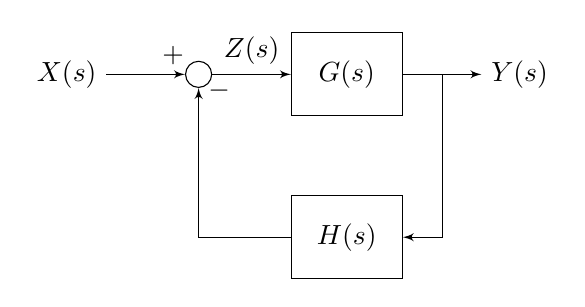
\begin{tikzpicture}[auto, >=latex']
    % Place the blocks
    \node [name=input] {$X(s)$};
    \node [sum, right=of input] (sum) {};
    \node [block, right=of sum] (G) {$G(s)$};
    \node [right=of G] (output) {$Y(s)$};
    \node [block, below=of G] (measurements) {$H(s)$};

    % Connect the nodes
    \draw [arrow] (input) -- node[pos=0.85] {$+$} (sum);
    \draw [arrow] (sum) -- node {$Z(s)$} (G);
    \draw [arrow] (G) -- node [name=y] {} (output);
    \draw [arrow] (y) |- (measurements);
    \draw [arrow] (measurements) -| node[pos=0.99, right] {$-$} (sum);
  \end{tikzpicture}

  \caption{Closed loop block diagram}
  \label{fig:closed_loop_deriv}
\end{figure}

\begin{align}
  Y(s) &= Z(s) G(s) \nonumber \\
  Z(s) &= X(s) - Y(s) H(s) \nonumber \\
  X(s) &= Z(s) + Y(s) H(s) \nonumber \\
  X(s) &= Z(s) + Z(s) G(s) H(s) \nonumber \\
  \frac{Y(s)}{X(s)} &= \frac{Z(s) G(s)}{Z(s) + Z(s) G(s) H(s)} \nonumber \\
  \frac{Y(s)}{X(s)} &= \frac{G(s)}{1 + G(s) H(s)}
\end{align}

A more general form is

\begin{equation}
  \frac{Y(s)}{X(s)} = \frac{G(s)}{1 \mp G(s) H(s)}
\end{equation}

where positive feedback uses the top sign and negative feedback uses the bottom
sign.

\section{Kalman filter as Luenberger observer} \label{sec:app_kalman_luenberger}

A Luenberger observer is defined as

\begin{align}
  \mtx{x}_{k+1}^+ &= \mtx{A} \mtx{x}_k^- + \mtx{B} \mtx{u}_k + \mtx{L}
    (\mtx{y}_k - \hat{\mtx{y}}_k) \label{eq:luenberger1} \\
  \hat{\mtx{y}}_k &= \mtx{C} \mtx{x}_k^- \label{eq:luenberger2} \\ \nonumber
\end{align}

where a superscript of minus denotes \textit{a priori} and plus denotes
\textit{a posteriori} estimate. Combining equation (\ref{eq:luenberger1}) and
equation (\ref{eq:luenberger2}) gives \\
\begin{equation} \label{eq:luenberger}
  \mtx{x}_{k+1}^+ = \mtx{A} \mtx{x}_k^- + \mtx{B} \mtx{u}_k + \mtx{L}
    (\mtx{y}_k - \mtx{C} \mtx{x}_k^-) \\
\end{equation}
\\
The following is a Kalman filter that considers the current update step and the
next predict step together rather than the current predict step and current
update step.

\begin{align}
  \text{Update step} \nonumber \\
  \mtx{K}_k &= \mtx{P}_k^- \mtx{H}^T (\mtx{H}\mtx{P}_k^- \mtx{H}^T +
    \mtx{R})^{-1} \\
  \mtx{x}_k^+ &= \mtx{x}_k^- + \mtx{K}_k (\mtx{y}_k - \mtx{H} \mtx{x}_k^-)
    \label{eq:post2_x} \\
  \mtx{P}_k^+ &= (\mtx{I} - \mtx{K}_k\mtx{H})\mtx{P}_k^- \\
  \text{Predict step} \nonumber \\
  \mtx{x}_{k+1}^+ &= \mtx{A} \mtx{x}_k^+ + \mtx{B} \mtx{u}_k
    \label{eq:pre2_x} \\
  \mtx{P}_{k+1}^- &= \mtx{A} \mtx{P}_k^+ \mtx{A}^T +
    \mtx{\Gamma}\mtx{Q}\mtx{\Gamma}^T
\end{align}
\\
Substitute equation (\ref{eq:post2_x}) into equation (\ref{eq:pre2_x}).

\begin{align*}
  \mtx{x}_{k+1}^+ &= \mtx{A} (\mtx{x}_k^- +
    \mtx{K}_k (\mtx{y}_k - \mtx{H} \mtx{x}_k^-)) + \mtx{B} \mtx{u}_k \\
  \mtx{x}_{k+1}^+ &= \mtx{A} \mtx{x}_k^- +
    \mtx{A} \mtx{K}_k (\mtx{y}_k - \mtx{H} \mtx{x}_k^-) + \mtx{B} \mtx{u}_k \\
  \mtx{x}_{k+1}^+ &= \mtx{A} \mtx{x}_k^- + \mtx{B} \mtx{u}_k +
    \mtx{A} \mtx{K}_k (\mtx{y}_k - \mtx{H} \mtx{x}_k^-) \\
\end{align*}

Let $\mtx{C} = \mtx{H}$ and $\mtx{L} = \mtx{A} \mtx{K}_k$.

\begin{equation} \label{eq:app_kalman_leunberger}
  \mtx{x}_{k+1}^+ = \mtx{A} \mtx{x}_k^- + \mtx{B} \mtx{u}_k +
    \mtx{L} (\mtx{y}_k - \mtx{C} \mtx{x}_k^-) \\
\end{equation}
\\
which matches equation (\ref{eq:luenberger}). Therefore, the eigenvalues of the
Kalman filter observer can be obtained by

\begin{align}
  &eig(\mtx{A} - \mtx{L}\mtx{C}) \nonumber \\
  &eig(\mtx{A} - (\mtx{A}\mtx{K}_k)(\mtx{H})) \nonumber \\
  &eig(\mtx{A}(\mtx{I} - \mtx{K}_k\mtx{H}))
\end{align}

\bibliographystyle{IEEEtran}
\bibliography{state-space-guide.bib}
\glsaddall
\printglossaries
\end{document}
